%*******************************************************************************
%****************************** Second Chapter *********************************
%*******************************************************************************

\chapter{Related Work}
\label{cha:related_work}

% **************************** Define Graphics Path **************************
\ifpdf
    \graphicspath{{Chapter3/Pics/Raster/}{Chapter3/Pics/PDF/}{Chapter3/}}
\else
    \graphicspath{{Chapter3/Pics/Vector/}{Chapter3/}}
\fi
This chapter starts with a presentation about available LISP platforms. Then, the first LISP monitor is presented, followed by a LISP manual management tool. After that, the focus will be on the open source LISP implementations and LISP use-cases. In the following, the challenges brought by LISP are illustrated. At last, we resume the LISP related studies and missing works.


%-< SECTION >--------------------------------------------------------------------
\section{LISP platforms}
\label{sec:platform}
Blabla 

%-< SUB SECTION >--------------------------------------------------------------------
\subsection{LISP Beta Network}
\label{subsec:platform_beta}
% \begin{itemize}[noitemsep,topsep=0pt]
%     \item First global LISP testbed.
%     \item Initiated by Cisco.
%     \item Introduce all its components: how many MR/MS, PxTR, etc.
% \end{itemize}

The first global LISP testbed called LISP Beta Network~\cite{lispbeta}~\cite{coras2014performance}, has been deployed since 2008. Started as the only LISP testbed, the LISP Beta network had a steady growth and achieved world-wide experimental deployment~\cite{lispCCR} with the purpose to gain real-life experience on LISP. Initiated by Cisco, the members of the LISP Beta Network are not only major companies and operators, but also academics, research laboratories, and startups offering LISP related services. Participants of this network are located in 34 different countries, with the highest concentration in Europe and North America.

The LISP Beta Network is composed of the mapping system, LISP routers (i.e., xTRs), mobile nodes, Re-encapsulating Tunnel Routers (RTR~\cite{ermagan2016nat}) and Proxy Tunnel Routers (PTR~\cite{rfc6832}). According to the latest architecture (October 2017)~\cite{lispbetaarchi}, LISP Beta Network has 7 available MR/MSes and 6 PxTRs. More precisely: 2 MR/MSes and 2 PxTRs are in US, 3 MR/MSes and 3 PxTRs are in Europe, 2 MR/MSes and 1 PxTR are in Asia. It mainly uses two EID addressing spaces: 153.16.0.0/16 for IPv4 and 2610:00D0::/32 for IPv6~\cite{lispCCR}, but there are also some other EIDs beyond them. On March \nth{14} 2012, the mapping system used by the LISP Beta Network has switched from LISP+ALT~\cite{rfc6836} to the more flexible LISP-DDT~\cite{lispDDT}. Changing the  mapping system has considerably reduced the configuration and maintenance burden, while a slight performance degradation has been observed~\cite{lispCCR}. % LISP Beta Network consists of 518 LISP sites\yue{Need to verify if still 518 now}. Although the deployment scope is still limited compared to the Internet, its size is sufficient to conduct reasonable measurement campaigns to understand LISP behavior and performance. 


%-< SUB SECTION >--------------------------------------------------------------------
\subsection{LISP-Lab platform}
\label{subsec:platform_lab}

% \begin{itemize}[noitemsep,topsep=0pt]
%     \item LISP-Lab is an open platform LISP testbed project.
%     \item Opened from 2015.
%     \item Already been interconnected to the LISP Beta Network with an Open-LISP DDT root~\cite{fuller2012lisp}.
% \end{itemize}

Due to a monolithic control by one single commercial actor, however, LISP Beta network has limitations to explore the innovative services. Thus, some other projects, such as ANR LISP-Lab project~\cite{lisplab}, are under implementation to develop new enhanced features.

LISP-Lab project aims at building an open platform, based on the LISP architecture, providing the environment to perform high quality research and support the design, development, and thorough assessment of new services and use-cases. LISP-Lab platform is solely deployed by the open source LISP implementation, using OpenLISP~\cite{OpenLISP}, opened to the external users from 2015. It is coordinated by a French consortium: two academic institutions (UPMC, TPT), two Cloud Networking SME (Alphalink, NSS), two network operators (Renater, Orange), two SMEs on Access/Edge Networking (Border 6, Ucopia) and one Internet eXchange Point (Rezopole). Ten international external partners are also joined the platform. At the moment of writing, LISP-Lab consists of 3 \acrshort{mr}s/\acrshort{ms}es and 2 PxTRs located in France, as well as 13 worldwide xTRs, and has already been interconnected to the LISP Beta Network with an Open-LISP DDT root~\cite{fuller2012lisp}.


%-< SECTION >--------------------------------------------------------------------
\section{LISP monitoring tools}
\label{sec:monitor}

%-< SUB SECTION >--------------------------------------------------------------------
\subsection{LISPmon}
\label{subsec:implementation_LISPmon}

% \begin{itemize}[noitemsep,topsep=0pt]
%     \item LISPmon is the only monitoring platform supervising the current LISP status.
%     \item How it works.
%     \item How to report its daily since early 2010.
% \end{itemize}
LISPmon is the only monitoring platform that supervises the current public LISP status, i.e., the mappings between the EID-prefixes and the \acrshort{rloc}s. This platform is developed by the Advanced Broadband Communications Center of UPC (Universitat Politècnica de Catalunya). It scans the whole IPv4 addressing space everyday, normally beginning at 7:00 a.m. (UTC), and queries them by sending the Map-Request to one specific MR of the LISP Beta network (i.e., 7 MRs are candidates to be selected). If this MR does not respond, it will choose another one as a replacement, and start the queries again, to guarantee that the reception of LISP Map-Replies changes smoothly % \yue{I don't understand 'changes smoothly' means what...}
between two consecutive days. The available EID-RLOC mapping information is published once per day, ever since the beginning of 2010.


% %-< SUB SECTION >--------------------------------------------------------------------
% \subsection{LISP-Views}
% \label{subsec:implementation_LISPViews}
% \yue{To be described in details later} We proposed this monitoring architecture and deployed it in 2016. LISP-Views is discussed in details in Chapter~\ref{cha:LISPViews}.

%-< SUB SECTION >--------------------------------------------------------------------
\subsection{LIG}
\label{subsec:implementation_lig}
% Description of LIG~\cite{rfc6835}.
\acrfull{lig}~\cite{rfc6835} is a LISP-specific manual management tool, used to obtain the mapping information for a certain EID by querying the LISP mapping system. It can be run by all devices that implement LISP, including xTR, PxTR, MR, MS, as well as by a host system at either a LISP-capable or non-LISP-capable site. A possible syntax for a LIG command could be:
\begin{equation}
lig <destination> [source <source>] [to <map-resolver>] \nonumber
\end{equation}
Where $<$destination$>$: is either a Fully Qualified Domain Name (FQDN) or a destination EID for a remote LISP site; source <source>: is an optional source EID to be inserted in the 'Source EID' field of the Map-Request; to $<$map-resolver$>$: is an optional FQDN or RLOC address for a MR. When LIG is launched, a Map-Request is sent for a destination IP address, and the returned Map-Reply is displayed as follows:
\begin{itemize}[noitemsep,topsep=0pt]
    \item The EID-prefix for the site that the queried destination EID matches.
    \item The locator address of the responder.
    \item The RLOC tuples $<$RLOC, Priority, Weight$>$.
    \item A round-trip-time (RTT) estimate for the Map-Request/Map-Reply exchange.
\end{itemize}

The remaining work for LIG is about processing of Negative Map-Replies: LIG should be able to clearly indicate how and why a Negative Map-Reply is received. Negative Map-Replies could be sent in the following cases: the LIG request was initiated for a non-EID address or there was rate-limiting on the responder.

%-< SUB SECTION >--------------------------------------------------------------------
\subsection{RIG}
\label{subsec:implementation_rig}
\acrfull{rig}~\cite{rfc8112} is also a LISP-specific manual management tool, but it is not like LIG, which can be served on top of any \acrshort{mds} to retrieve RLOCs used for packet encapsulation. RIG is used to recursively find all the \acrshort{ms}es serving an EID-prefix, specifically within a \acrshort{lispddt} mapping database framework. It performs the same operation as that of a \acrshort{mr}. More specifically, when RIG command is run, a Map-Request is sent into the DDT hierarchy for a destination EID, and is forward based on the EID-prefix and delegation referrals contained in the Map-Referral messages until the DDT \acrshort{ms} containing the mapping information is reached. It can be run on the same devices as LIG. A simple syntax for a RIG command could be:
\begin{equation}
rig <eid> to <ddt-node> [follow-all-referrals] \nonumber
\end{equation}
Where $<$eid$>$ is the destination EID being queried; $<$ddt-node$>$ is the RLOC of any DDT node in the DDT hierarchy; when the keyword $[$follow-all-referrals$]$ is used, all the referral RLOCs will be queried; if this keyword is not used, one of the referral RLOCs will be selected to descend a branch of the DDT hierarchy. The results of returned Map-Referral messages mainly contain the RLOCs of child nodes storing the destination EID mapping information, as well as RTT indicating the time spends for getting the referral DDT nodes.


%-< SECTION >--------------------------------------------------------------------
\section{LISP implementations}
\label{sec:implementation}
% \begin{itemize}[noitemsep,topsep=0pt]
%     \item There are several proprietary LISP implementations, used on Cisco routers and on AMV's FRITZ!Box home routers. 
%     \item In this subsection, we introduce some open source LISP implementations.
% \end{itemize}
There are several proprietary LISP implementations. The most widely used are the implementations on Cisco routers and on AVM's FRITZ!Box home routers~\cite{AVMFritzBox}. Both can be used to test LISP and connected with the LISP Beta Network. However, the source codes of their implementations are not available and thus cannot be extended for LISP research purposes. Thus, in this section, we focus on some open source LISP implementations, which can help the researchers verify their improvements so to move forward LISP technology.


%-< SUB SECTION >--------------------------------------------------------------------
\subsection{OpenLISP}
\label{subsec:implementation_OpenLISP}
% Description of OpenLISP~\cite{OpenLISP}~\cite{phung2014openlisp}.
OpenLISP~\cite{OpenLISP}~\cite{phung2014openlisp} is an open source implementation of LISP protocol. The LISP Data Plane, such as: LISP-Cache and LISP-Database, as well as the encapsulation/decapsulation functions are implemented in the kernel of FreeBSD~\cite{freeBSD} Operating System. LISP Control Plane is written in C in the user space of FreeBSD and Linux. Everything related to the Control Plane is meant to run in the user space. OpenLISP does not provide any specific control plane protocol implementation associated to mapping distribution protocol. Instead, it implements a new type of sockets, called the Mapping Sockets providing an API that can be used by any users space process. OpenLISP was implemented by researchers from Universite catholique de Louvain and T-Labs/TU Berlin. At the moment of writing, Pierre et Marie Curie University maintains the Lip6-lisp~\cite{lip6lisp}, which is an extended implementation of OpenLISP and it supports fully featured LISP Control-Plane.


%-< SUB SECTION >--------------------------------------------------------------------
\subsection{OOR}
\label{subsec:implementation_oor}
% Description of Open Overlay Router (OOR)~\cite{OOR}.
Open Overlay Router (OOR)~\cite{OOR}, the successor of LISPmob~\cite{cabellos2011lispmob}, is an open source LISP and LISP mobile node implementation written in C for Linux, Android (only on rooted devices) and OpenWrt that uses LISP or VXLAN~\cite{mahalingam2014virtual}/GRE~\cite{hanks2000generic} as an overlay for SDN. LISPmob was initially developed by Cisco. By interoperating with LISP Beta Network, LISPmob enables mobile hosts to change its network attachment point without losing connectivity, while maintaining the same IP addresses. Now OOR is maintained by Barcelona Tech University. It focus on supporting for network function virtualization (NFV), e.g., by SFC, and integration with OpenDaylight~\cite{OpenDaylight}. The extended feature set makes OOR attractive for application.


%-< SUB SECTION >--------------------------------------------------------------------
\subsection{PyLisp}
\label{subsec:implementation_pylisp}
% Description of pylisp~\cite{pylisp}.
PyLisp~\cite{pylisp} is a small but functional implementation of LISP in Python. There is a packet of PyLisp implementation on Github, called pylisp~\cite{pylispgithub} provides the means to parse and create LISP data and control messages, as well as command line tools to perform actions like asking a map resolver for a mapping. The functions of PyLisp are not complete, so the intention to the later stage is the implementations for map server, map resolver and DDT node.


%-< SUB SECTION >--------------------------------------------------------------------
\subsection{jLISP}
\label{subsec:implementation_jLISP}
% Description of jLISP~\cite{stockmayer2016jlisp}.
jLISP~\cite{stockmayer2016jlisp}, proposed in 2016, is an open source implementation of LISP in Java and runs in the user space. It is platform-independent and object-oriented. jLISP is compatible with the LISP RFCs and is modular, which facilitates to explicit programs for every LISP component, such as: xTRs, RTRs, NTRs, and the mapping-system.


%-< SUB SECTION >--------------------------------------------------------------------
\subsection{LISP on OMNet++}
\label{subsec:implementation_OMNet}
% Description of the simulation model~\cite{klein2012integration} on OMNet++.
This implementation is a simulation model, which integrates LISP into the INET framework~\cite{klein2012integration} for OMNeT++~\cite{omnetpp}. It includes basic LISP functions, interworking mechanism, \acrshort{lispmn} architecture with its different update mechanisms, and their proposed NAT traversal mechanism. Since this simulation model is proposed in 2012, the mapping system is LISP-ALT instead of nowadays LISP-DDT. This would be an obstacle for this implementation that is widely used now\yue{OMNeT++ is open source. but the paper does not mention if their simulation model is open source or not}.


% %-< SUB SECTION >--------------------------------------------------------------------
% \subsection{LISP on NS3}
% \label{subsec:implementation_NS3}
% \yue{To be described in details later} We proposed in 2017 and described in depth in Chapter~\ref{cha:ns-3}.




%-< SUB SECTION >--------------------------------------------------------------------
\subsection{Lispers.net}
\label{subsec:implementation_lispers}
% Description of Lispers.net~\cite{lispers}.
Lispers.net~\cite{lispers} is a Python implementation aiming to implement the complete feature set of LISP. Additional non-LISP-specific functions and behaviors are added, which make lispers.net a general overlay controller. Until December \nth{27} 2017, the latest version of lispers.net is Beta Release Version 0.430.







%-< SUB SECTION >--------------------------------------------------------------------
\subsection{LISP controller in ONOS}
\label{subsec:implementation_onos}
%-< FIGURE >--------------------------------------------------------------------
\begin{figure}[!t]
	\centering
	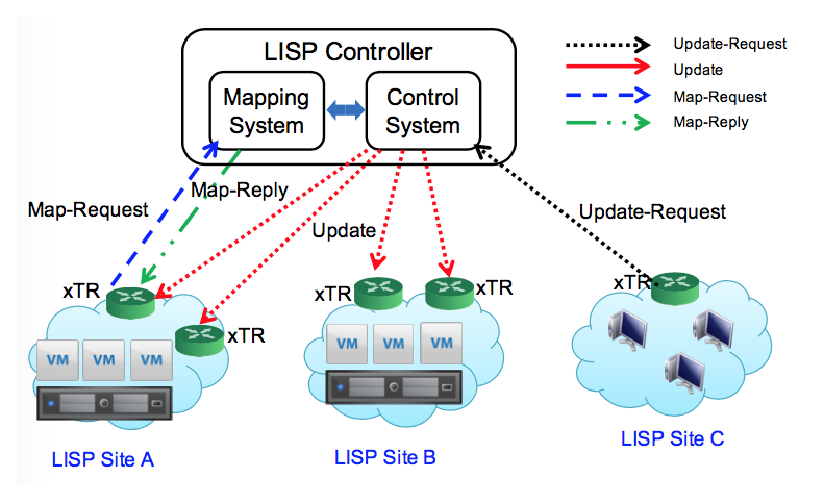
\includegraphics[width=\textwidth]{Pics/concept_of_LISP_controller.eps}
	\caption{The concept of LISP controller (source:~\cite{han2016design})}
	\label{concept_of_LISP_controller}
\end{figure}
%-< END FIGURE >--------------------------------------------------------------------
The LISP controller in Open Network Operating System (ONOS), which is an open source SDN OS for service providers~\cite{han2016design}, is one of South Bound Interfaces (SBI) for SDN controllers. The LISP controller in ONOS is proposed to address the OpenFlow issues, such as: scalability, performance, heterogeneity, inter-operability with legacy networks and protocols. An open source SDN controller development project, called OpenDaylight~\cite{OpenDaylight} sub-project, is developing the LISP mapping system in SDN environments. The LISP controller centralizes LISP controls into a single entity. It supports LISP as an SDN SBI to work with other protocols such as OpenFlow, and provides APIs for LISP applications. The concept of LISP controller is depicted in Fig.~\ref{concept_of_LISP_controller}. The LISP controller brings many benefits, such as: simplified management, a global view of LISP networks, short information convergence time, and easy development support of LISP based applications. 


\label{subsec:related_studies}
% Summarize all LISP-related studies:
\section{LISP impact and challenges}
\label{subsec:studies_impact}
%-< SUBSUB SECTION >--------------------------------------------------------------------
\subsection{The maximum transmission unit (MTU) issue}
\label{subsubsec:impact_mtu}
LISP encapsulation adds 36 bytes for IPv4 (i.e., 20 bytes of outer header + 8 bytes of UDP header + 8 bytes of LISP header) and 56 bytes for IPv6 (i.e., 40 bytes of outer header + 8 bytes of UDP header + 8 bytes of LISP header) to the original packet size. As with other protocols that encapsulate or tunnel traffic (e.g., IP Security (IPsec)~\cite{thayer1998rfc} and generic routing encapsulation (GRE)~\cite{farinacci2000generic}), it is possible that the resultant encapsulated packets would exceed the permissible MTU somewhere along the transit path. LISP provides both stateful and stateless mechanisms for handling potential MTU issues~\cite{CiscoLISPQA}, with the main goals being 
\begin{enumerate*}[label=(\roman*)]
  \item preventing packets from being dropped, and
  \item preventing the need for ETRs to perform packet reassembly prior to LISP de-encapsulation. 
\end{enumerate*}

Based on real Internet experiments, \cite{lispCacheCost} and \cite{kim2013caching} show that although the encapsulation overhead is not negligible, it is very limited (in the order of few percentage points of the total traffic volume). In addition, no major issue due to the MTU is observed on the LISP Beta Network.

%-< SUBSUB SECTION >--------------------------------------------------------------------
\subsection{Impact on traffic between LISP-site and the legacy Internet}
\label{subsubsec:impact_pxtr}
LISP has no impact on traffic to nowadays legacy Internet if neither source nor destination is LISP. However, it has significant impact on the traffic between LISP-site and non-LISP-site. First, to support the interworking between LISP-site and the legacy Internet, the PxTRs should be set up. The configuration on \acrshort{pxtr} does not cause any special technical issue, but using \acrshort{pxtr} potentially causes path stretch between source and destination. It makes the packet exchange experience a larger delay and potentially leads to higher packet loss rate. Thus, placing the PxTR near the source of traffic allows the communication between the non-LISP site and the LISP site to have the least path stretch (i.e., the least number of forwarding hops when compared to an optimal path between the sites)~\cite{rfc6832}. Moreover, as PxTRs advertise in BGP the EID-prefixes that they are behalf of, if they are managed by different entities (i.e., they belong to different ASes), it is possible to cause MOAS (Multi-Origina AS) issues~\cite{rfc7834}.

When deploying the PxTRs in the experimental infrastructure, it is better to think about first where to deploy the PxTRs, since the placement in topology has a significant impact on the path stretch. Besides, as the number of PxTRs has a direct impact on the traffic load and the recovery success in case of the failure of a PxTR, we need consider how many PxTRs are needed. Further, we need to think if all the PxTRs advertise for the whole EID space or each of them just announces for the different segmented EID-prefixes.

%-< SUBSUB SECTION >--------------------------------------------------------------------
\subsection{Troubleshooting problem}
\label{subsubsec:impact_troubleshooting}
A big issue in the LISP experimentation is the difficulty of troubleshooting. The most frequent used troubleshooting tool is \emph{traceroute}, but it can not provide the exact path that the packets pass between the xTRs or PxTRs. The experimenters only know how many hops between them. When the host traceroutes a destination, it uses each EID as the source/destination IP address of ICMP. However, when the packets pass to the \acrshort{itr}, it encapsulates the packets, so the following routers think that the \acrshort{itr} is the source of ICMP and will give back the ICMP message to the \acrshort{itr}. In this way, the host, which is the real source launching the ICMP receives no response. Until the packets reach to \acrshort{etr} or \acrshort{petr}, they dencapsulate the packets to know the real source of ICMP and answer to the EID of host.

%-< FIGURE >--------------------------------------------------------------------
\begin{figure}[!t]
	\centering
	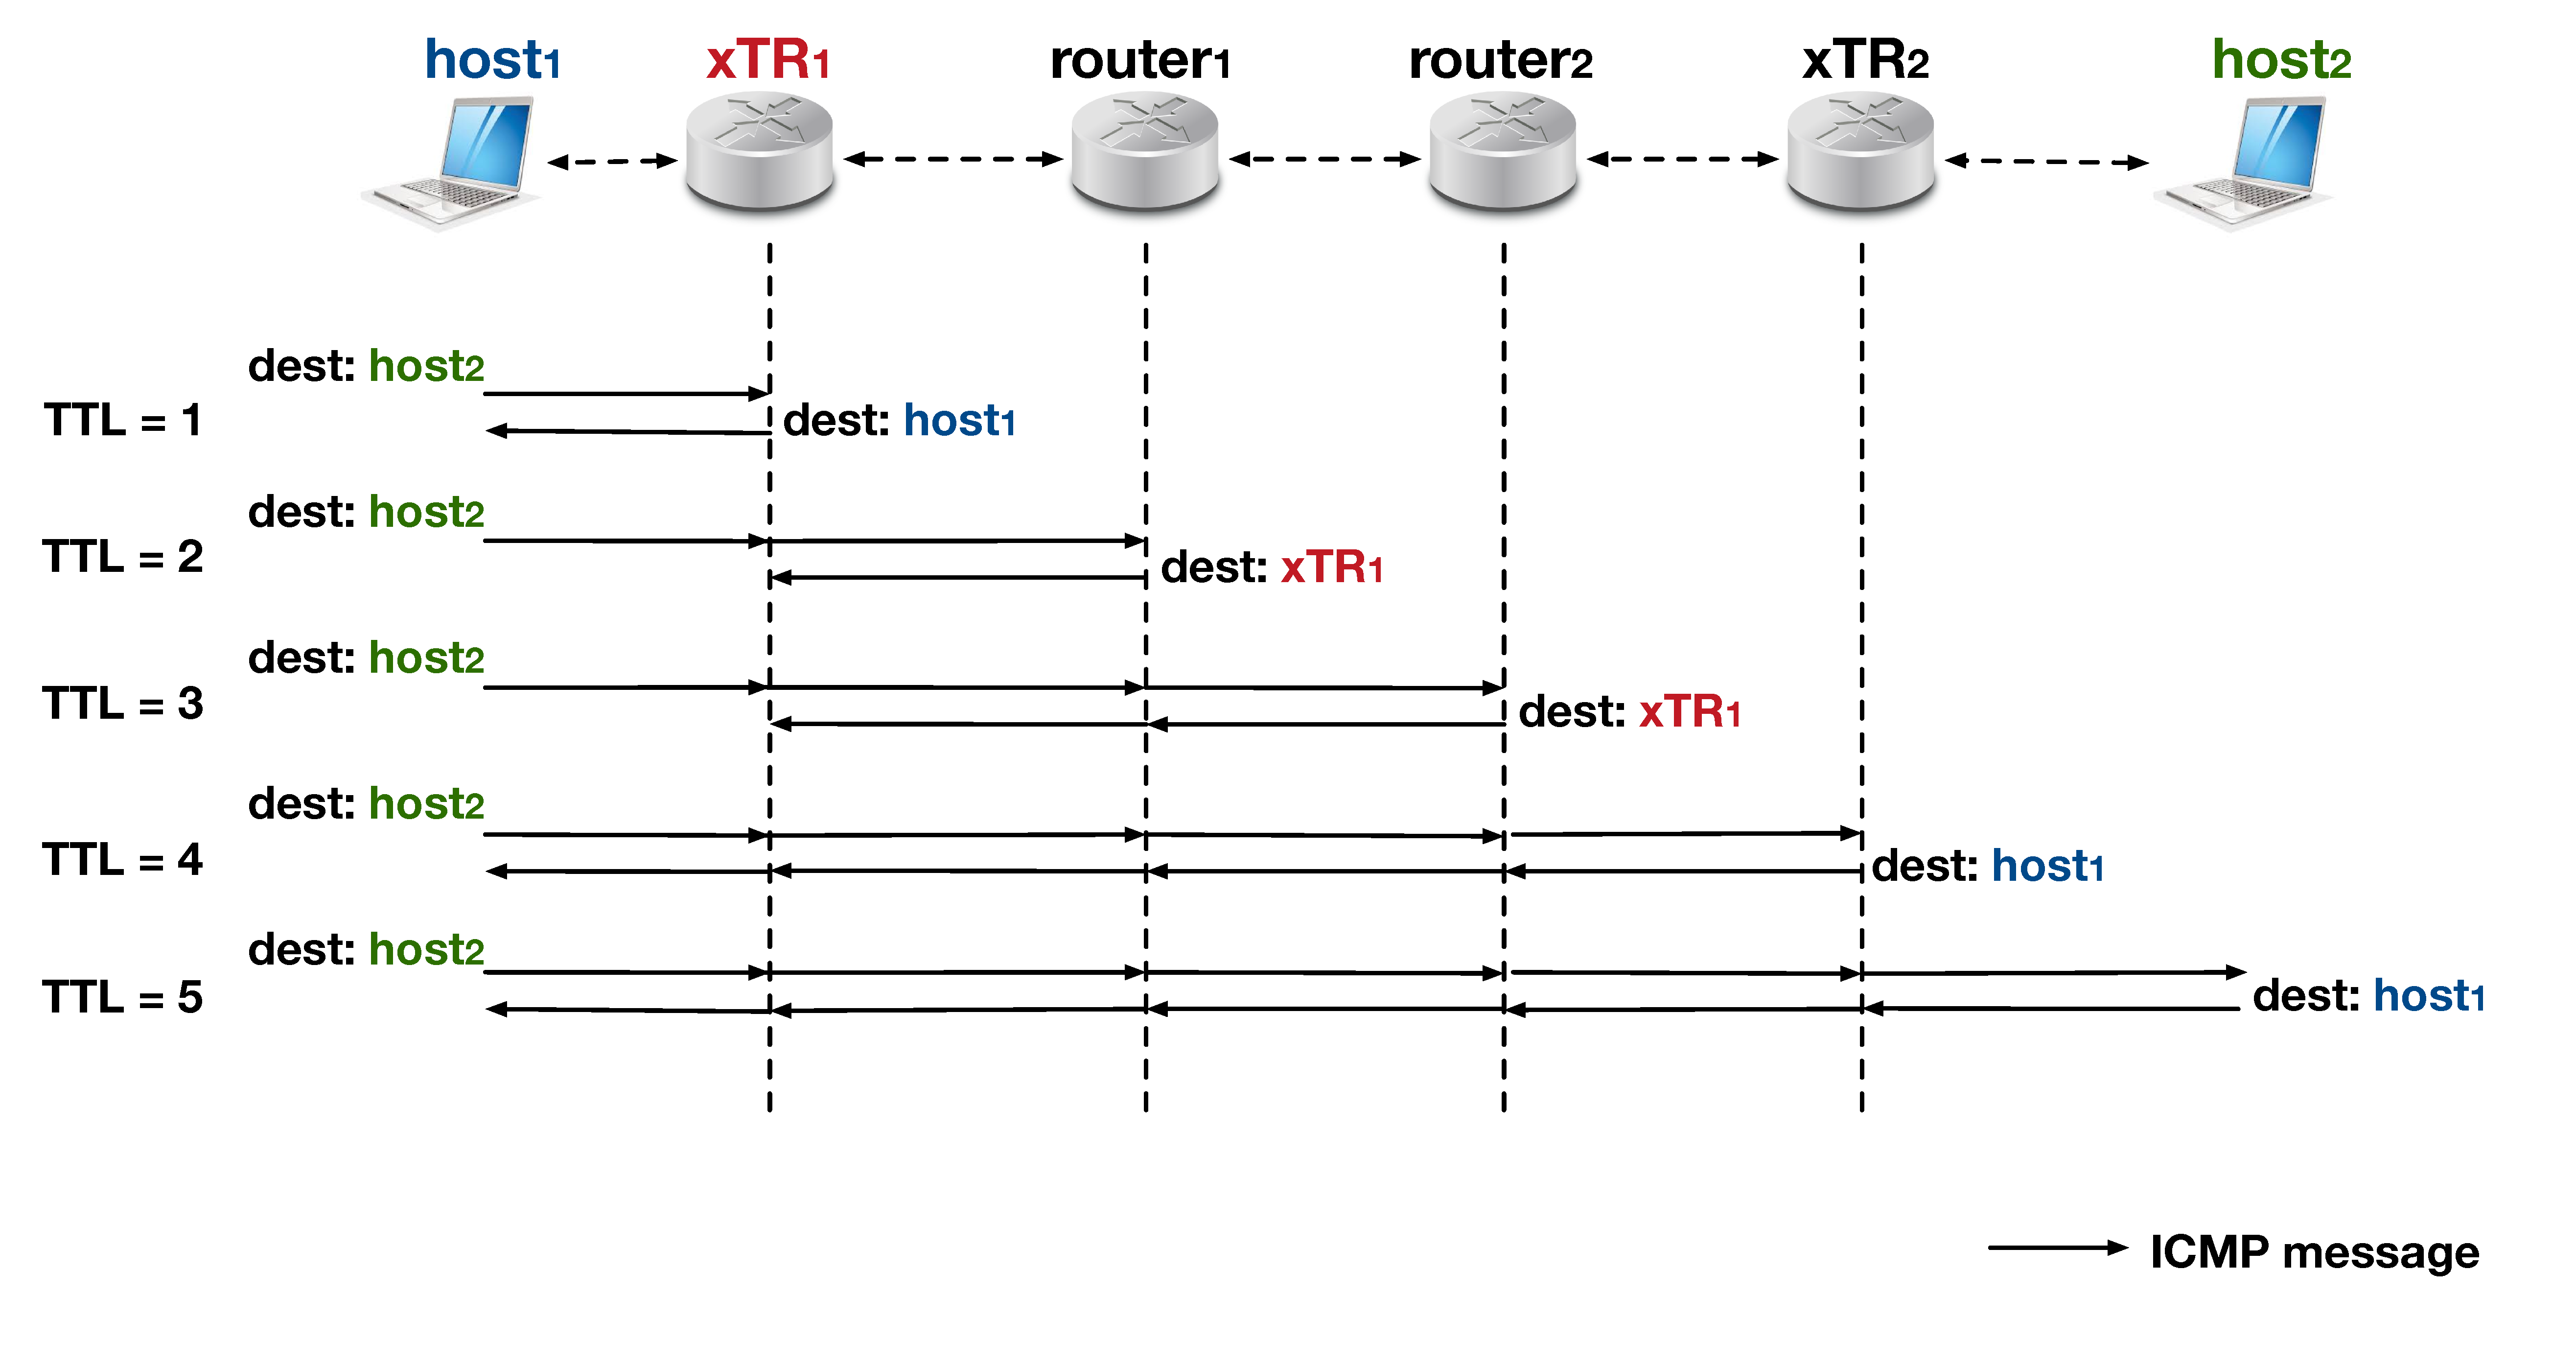
\includegraphics[width=\textwidth]{Pics/LISP_traceroute.eps}
	\caption{Illustration of LISP troubleshooting}
	\label{Illustration_LISP_troubleshooting}
\end{figure}
%-< END FIGURE >--------------------------------------------------------------------
An example of LISP troubleshooting is shown in Fig.~\ref{Illustration_LISP_troubleshooting}. When $host_1$ traceroutes $host_2$, the first ICMP message with TTL (time-to-live)=1 expires at $xTR_1$, then it sends back the ICMP Time Exceeded message to $host_1$. When $xTR_1$ receives the ICMP message with TTL=2, it decreases the TTL value, encapsulates the ICMP message with its own RLOC as source address and forwards to the next hop $router_1$. Since the ICMP message that the $router_1$ receives showing $xTR_1$ is the source instead of $host_1$, the $router_1$ drops the packets and replies back to $xTR_1$. In this way, the $host_1$ cannot receive any ICMP Time Exceeded messages until the $xTR_2$ is tracerouted. When the $xTR_2$ receives the ICMP message, it denpsulates the packets and finds that the real traceroute sender is $host_1$. Thus the $xTR_2$ replies to $host_1$. Same to $host_2$, the received ICMP message shows that $host_1$ is the traceroute origin and itself is the destination, so it returns an ICMP Echo Reply message $host_1$. 

To the conventional Internet topology, \emph{traceroute} uses the returned ICMP Time Exceeded messages to build a list of routers that packets traverse until the destination is reached. However, due to the troubleshooting problem LISP facing to, the list of routers between xTRs is hidden to the traceroute sender. It can only know how many hops it needs to arrive the ETR. Thus, when there is a problem in the LISP network, it is hard for the operators to pinpoint the reason as they have only a partial view of the network. The experimenters can leverage on the LISP Cache/Database or querying the \acrshort{mr}s to observe the potential problem in the network, but the knowledge remains limited. 

%-< SUBSUB SECTION >--------------------------------------------------------------------
\subsection{LISP security}
\label{subsubsec:impact_security}
As LISP is born to address the scalability issues of Internet, it is not designed for the security by nature. The possible security threats with that LISP are faced are given in~\cite{rfc7835}. Although after the authentication, the \acrshort{ms}es only accept the registrations of their compromised ETRs, the compromised ETRs may de-aggregate their EID-prefixes in order to register more EID prefixes than necessary to their \acrshort{ms}es, so to cause overwhelmed Map-Requests. The compromised ETRs may also overclaim the prefix they own in order to influence the route followed by Map-Requests for EIDs outside the scope of their legitimate EID-prefix. Besides, the Map-Register stage is vulnerable to masquerading and content poisoning attacks, for example: the ETRs register the fake mapping information to the \acrshort{ms}es~\cite{aiash2013securing}~\cite{montero2013securing}~\cite{aiash2013novel}. By sending the Map-Requests at a high rate can overload the nodes in the MDS and cause the flood of Map-Replies as well. Some bits in the LISP control plane messages also have some security issues, for example: the Locator-Status-Bits can cause a DoS (Denial-of-Service), a replay, a packet manipulation, or a packet interception and suppression attack; the Map-Version number can mount a DoS, an amplification, or a spoofing attack; the routing locator reachability is able to mount a packet manipulation and an amplification attack.

A set of security mechanisms (LISP-SEC) that provides authentication, integrity and anti-replay protection for LISP are introduced in~\cite{maino2017lisp}. A number of vulnerabilities should be considered before deploying LISP in large scale~\cite{raheem2013supporting}.


%-< SUB SECTION >--------------------------------------------------------------------
\section{LISP Related studies and missing works}
\label{subsec:studies_status}
% Summarize the latest LISP status from research papers

% %-< SUB SECTION >--------------------------------------------------------------------
% \subsection{LISP measurement results}
% \label{subsec:studies_status}

\subsection{LISP Cache performance}
\label{subsec:lisp_cache}
A thorough analysis of LISP Cache is presented in~\cite{lispCacheCost},~\cite{lispCacheDive} and~\cite{kim2013caching}. Their works complement and validate each other. The papers %analyzes two 24-h traces of a large European ISP and shows 
show that although the cache time largely reduces from initial 24-h to as small as 60s, the LISP cache maintains a very high efficiency, with more than 99\% hit-ratio. As a result, the cache highly reduces the size, and the traffic volume overhead introduced by both the traffic encapsulation and the control traffic to request missing mappings is limited to 6\%. Around 70\% of cache missing, it is generated by UDP protocol regardless the port number. The authors argue that is mainly caused by P2P applications or any other distributed applications generating the same spread traffic pattern. They also compare the the original LISP specification, called vanilla LISP with the symmetric LISP model, proposed by Saucez et al., and show that the later model provides higher security. Besides, they evaluate the relationship between the size of cache and the number of users. It shows that when the number of users is increased to three times, the size of cache is only double. It means that the average size of the LISP Cache is not linear relationship with the number of hosts.

\subsection{LISP Mapping System evaluation}
\label{subsec:lisp_mds}
The performance of LISP Mapping System is evaluated in~\cite{lispCCR} and~\cite{coras2014performance} from different aspects. As the LISP Beta Network changed its mapping system from LISP+ALT to LISP-DDT on March \nth{14} 2012, the authors measure the delay of resolving mapping (the latency between sending the Map-Request and receiving the Map-Reply) during this transition period. They find the delay to get the mapping by using LISP+ALT is smaller and more stable than LISP-DDT. However, the manageability of the later is better than the former, since by using LISP+ALT, the Map-Requests normally need traverse the entire BGP overlay and maintaining the ALT also causes many cumbersome overheads especially as the network growing. Although using LISP-DDT slightly degrades the resolving mapping performance, but the delays are rather small and the mapping system is able to cope with a significant growth of the addressing space. The resolution delay is slightly various from the vantage points and the \acrshort{mr}s, but the European infrastructure is unreliable due to the loss of many queries.

\subsection{LISP network evolution}
\label{subsec:lisp_evolution}
After deploying LISP in LISP Beta Network from 2008, more and more participants attended to the development of LISP. The LISP network is steady flourishing. Thus, the paper~\cite{lispCCR} looks at how the LISP network evolves. The authors observe that the number of LISP mapping was as low as 20 in January 2010, but it has consistently grown to reach 80 mappings in 2012. The number of LISP mappings is four times to the initial number, which indicates that LISP network has a regular growth. Within two months of the second part of 2011, the number of negative mappings was doubled, i.e., from about 150 to about 300. The authors suppose that is due to a more fragmented EID-space. The paper also observes some malformed mappings, which belongs to the LISP mappings but have an empty RLOC set. However, this kind of mappings is never more than 0.5\% of the total number of mappings within one day. Further, the paper presents that from January 2010 to May 2012, the percentage of mappings using two or less RLOCs has increased. Moreover, there exists mappings with four RLOCs in 2012, whereas they were not present in January 2010.

\subsection{LISP interworking}
\label{subsec:lisp_interworking}
As more and more deployments of LISP, it becomes necessary that the LISP networks communicate with the legacy Internet. The evaluation of the interworking performance is presented in reference~\cite{coras2014performance}. It chooses 200 \acrshort{vp}s on the PlanetLab (a global research network that supports the development of new network services from 2003)~\cite{PlanetLab} located in North America, Asia and Europe by the order of diversity of number of \acrshort{vp}s. It also selects 116 EIDs, which have at least 1 corresponding RLOC in the mapping from the daily of LISPmon project~\cite{lispmon} published on May \nth{17} 2013. The experiment is conducted from November \nth{4} to \nth{7} 2013. The authors find that the interworking generally has a negative impact compared to without using LISP. The results show that there are 70\% of the EID-prefixes have at least 20\% of increase in the delay (i.e., \acrfull{rtt}). One \acrshort{pxtr} behaves the worst that 95\% of the EID-prefixes using it suffer from a delay increase. Based on BGP, the selection of \acrshort{pitr}s is driven by the economical relationship between autonomous systems, instead of their geographical positions. As a result, even if the LISP Beta Network has 9 available \acrshort{pxtr}s at the moment, there are only 4 are used in the experiment. Further, the most \acrshort{vp}s use \acrshort{pxtr}s in Asia although they are located in Europe or America. The most popular \acrshort{pxtr} is selected 79\% of times.


\subsection{LISP mobility}
\label{subsec:lisp_mobility}
% \yue{Support for Network-based User Mobility with LISP}
To support IP mobility, the conventional LISP should be extended. The first mobility-compatible LISP extension is LISP-MN~\cite{mn00}\cite{natal2013lisp}. LISP-MN is an end-host based IP mobility protocol which requires updating the software of the mobile terminal. In other words, the end-host that uses LISP-MN can be regarded as a small LISP site.

The main drawbacks of LISP-MN are the double encapsulation and the need to modify software in end-host. Double encapsulation could increase mapping latency, overhead and MTU issues. The modification at end-host hinds the deployment of LISP-MN. To overcome these drawbacks, lots of research efforst are made by LISP community.

The performance of LISP-MN is investigated in a qualified way in~\cite{menth2010improvements}. The authors illustrate the performance degradation due to double encapsulation and the triangle route problem under some conditions. They also propose mechanisms such as location-aware LISP mobility node, local mapping systems to improve the performance of LISP-MN. A simple model that help analyze the handoff procedure in IP mobility is proposed by~\cite{phoomikiattisak2016control}. Besides LISP-MN, the proposed model can be also used for the handoff analysis for other IP mobility protocols such as MIPv6. 

To avoid the modification to end-host required in LISP-MN, a network-based and LISP-based IP mobility protocol: LISP-ROAM is proposed in~\cite{galvani2014lisp}. Their solution is that the network assigns the same IP address regardless of their network attachment point under the cooperation between some additional/modified network components (DHCP servers, authentication services, LISP xTR and servers). The authors implement LISP-ROAM on top of LISPmob and give an experimental evaluation of the performance of LISP-ROAM. As an effort to avoid double encapsulation in LISP-MN, LISP-NEMO is proposed in~\cite{wu2014nemo}. The basic idea of LISP-NEMO originates from NEMO~\cite{jeon2010network}. It introduces a new network element called mobile router (MR) that manages and represents the mobile network. To mitigate the problems in LISP-NEMO and LISP-ROAM, LISP-HNM is proposed in~\cite{tang2017lisp}. The authors introduce an access register protocol and an active
notification scheme to conventional LISP so that the latter can support both end-host and network mobility.

The packet loss due to IP mobility is also a concern. To reduce the packet loss, Isah et al.~\cite{isah2017towards} propose an improvement to LISP-MN. The basic idea is that those packets generated during handover procedure are buffered to severs close to the MN’s new location and forwarding them to the MN on handover completion.

% Essentially conceived for mobile equipment, LISPmob could also be installed in the VM; there would be, however, a problem with most current hypervisors that impose the VM external address to be in the same subnet before and upon migration, which practically limits the LISPmob usability only to situations where source and destination networks are either LISP sites themselves, or layer-2 over WAN solutions. In the first case, a double encapsulation is needed, which could increase mapping latency, overhead and MTU issues. There may also be scalability issues with a high VM number.




\subsection{LISP security proposal}
\label{subsec:lisp_sec_proposal}
The Sec.~\ref{subsubsec:impact_security} of Chapter 3 indicates that LISP faces some secure threats~\cite{raheem2013supporting}~\cite{montero2013securing}. The reference~\cite{aiash2013novel} analyses the security and functionality of the LISP mapping procedure using a formal methods approach based on Casper/FDR tool. The authors point out several security issues in the protocol such as the lack of data confidentiality and mutual authentication. The reference~\cite{aiash2013securing} figures out that the Map-Registration stage is vulnerable to masquerading and content poisoning attacks. Therefore, it presents a new security method for protecting the LISP Registration stage. The proposed method uses the ID-Based Cryptography (IBC), which allows the \acrshort{mds} to authenticate the source of the data. 


%-< SUB SECTION >--------------------------------------------------------------------
\subsection{LISP missing works}
\label{subsec:studies_status}
% Highlight what is missing in those works.

As querying the mapping information to the \acrshort{mds} largely increases packet transmission delay, to store the necessary mappings in the LISP Cache can significantly alleviate it. However, as limited capacity of LISP Cache and dynamic changes of mapping information, it still requires smart algorithms to determine which mappings should be reserved or removed for better performance, especially when there are many expired mappings caused by mobility~\cite{feng2017locator}.

The previous measurements of the \acrshort{mds} are mainly depended on the delay, including the different resolving latency that each \acrshort{mr} needs to use, and comparing which \acrshort{vp}s have longer delay to query the mappings. However, the authors have never taken look at the contents of mapping information. Precisely, there is no work to compare whether the consecutively received Map-Replies change, neither the comparisons on the Map-Replies sent by the different \acrshort{mr}s nor received by the different \acrshort{vp}s for the same \acrshort{eid}s are same.

The only evaluation of PxTR used for the interworking between LISP and legacy Internet was conducted in 2013. At that time, the unique LISP platform was the LISP Beta Network. Thus, the measurement was only based on its PxTRs and the \acrshort{vp}s on the research network PlanetLab. After the open of LISP-Lab platform in 2015, there is no evaluation about the PxTR anymore. We do not know the recent performance of PxTR on LISP Beta Network and we have no knowledge about if the PxTR of LISP-Lab function well. Further, the previous assessment was conducted within an experimental/research environment, there is no experience about the interworking performance in the realistic network, especially for the interoperability with the current popular websites on the world.

LISPmon as the first and only LISP monitor satisfies the preliminary LISP requirements at the initial stage, but faces some limitations as the quick development of LISP. LISPmon just publishes the mapping information as the daily once per day. All the published results are queried to one \acrshort{mr} of LISP Beta Network and captured on one \acrshort{vp}. Since LISP Beta Network has multiple \acrshort{mr}s over the world and the join of LISP-Lab platform later, the current monitoring mechanism of LISPmon shows the incompleteness. To move LISP forward, it is necessary to fully understand the performance of every LISP network entity. Beyond only publishing the mapping information between EID-prefix and its \acrshort{rloc}s, automatically conducting the comprehensive experiments from the various aspects will help the LISP experimenters improve their research speed and enrich their study fields.

At the moment, LISP has some implementations for the different Operation Systems, including either the proprietary source or the open source. However, LISP always lacks of an open source simulator, which is much easier and more flexible for the researchers to test the new features.

To achieve the seamless handover, LISP can be implemented on the border router or directly on the host to support the mobility. However, these proposals are only limited at the theoretical level. There are no experimental results show which solution is better based on such as the smaller handover delay or the less packet loss. No evaluations respectively introduce the advantages and the disadvantages of each solution. What's more, no matter which solution is adopted to conduct the mobility, SMR and Map-Versioning are the candidates to revoke the remote ITR to update its mapping cache. Thus, it is interesting to make a comparison between these two mechanisms, for example modeling the overhead traffic according to the number of \acrshort{mn}s and \acrshort{cn}s of each mechanism.